As the Stack we already know the basic operations of a Queue, so we have an idea about what we go to program, but what is the structure of a Queue? As I mentioned before maybe show a draw or schema is better to understand what we need to program so I have maked a little draw of how I imagine a Queue.

\begin{figure}[H]
    \centering
    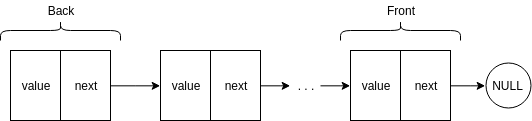
\includegraphics[width=1.00\textwidth]{Images/DataStructures/Queue/Queue.png}
    \caption{Diagram of a Queue}
    \label{fig:queue_diagram-01}
\end{figure}

As you can see a stack has a ''back'' and ''front'' element where ''back'' is the last element of the queue and ''front'' is the first element. Each element (lets call them as nodes) has a value and a pointer to the next element, if we wrote this using code we have the next result:

\begin{lstlisting}
    #include <bits/stdc++.h>

    using namespace std;

    struct Node{
        int value;
        Node *next;

        Node( int _value ){
            value = _value;
            next = NULL;
        }
    };

    struct Queue{

        Node *back;
        Node *front;
        int size;

        Queue(){
            back = front = NULL;
            size = 0;
        }

        void Enqueue( int value ){
            Node *node = new Node( value );
            if( size == 0 )
                back = front = node;
            else {
                node -> next = back;
                back = node;
            }

            size++;
        }

        void Dequeue(){
            Node *aux = back;
            if( size > 1 ){
                
                while( aux -> next != NULL )
                    aux = aux -> next;

                aux -> next = NULL;
                front = aux;

            } else if( size == 1 )
                front = back = NULL;
            else 
                return;
            size--;
        }

        bool IsEmpty(){
            return (size == 0);
        }

        int Top(){
            return (front -> value);
        }

        int GetSize(){
            return size;
        }
        
        void print(){
            cout << endl;
            Node *aux = back;
            while( aux != NULL ){
                cout << aux -> value << " ";
                aux = aux -> next;
            }
            cout << endl;
        }
    };
\end{lstlisting}

\subsection{Problems}
\subsubsection{Problem 01}
\textsf{Implement a stack using a queue}
\begin{lstlisting}
    #include <bits/stdc++.h>

    using namespace std;

    int main(){
        string s;
        int number_01 = 0, number_02 = 0;
        stack< int > Stack;
        cin >> s;

        for( auto c : s ){
            if( isdigit(c) ){
                Stack.push( c - '0' );
            } else {

                number_01 = Stack.top();
                Stack.pop();
                number_02 = Stack.top();
                Stack.pop();

                if ( c == '+')
                    Stack.push( number_02 + number_01 );
                else if ( c == '-' )
                    Stack.push( number_02 - number_01 );
                else if ( c == '*' )
                    Stack.push( number_02 * number_01 );
                else if ( c == '/' )
                    Stack.push( number_02 / number_01 );
            }
            
        }
        cout << Stack.top() << endl;
        return 0;
    }
\end{lstlisting}

\subsubsection{Problem 02}
\textsf{Reverse first k elements of a queue}
\begin{lstlisting}
    #include <bits/stdc++.h>

    using namespace std;

    stack< int > StackSort(stack<int> &Stack){

        stack<int> AStack;
        
        while( !Stack.empty() ){
            int aux = Stack.top();
            Stack.pop();
            
            while( !AStack.empty() && AStack.top() > aux ){
    
                Stack.push( AStack.top() );
                AStack.pop();    

            }

            AStack.push( aux );
        }
        return AStack;
    }

    int main(){
        stack<int> Stack;
        int n, v;
        cin >> n;
        while(n--){
            cin >> v;
            Stack.push(v); 
        } 

        Stack = StackSort( Stack );

        while( !Stack.empty() ){
            cout << Stack.top() << endl;
            Stack.pop();
        }

        return 0;
    }
\end{lstlisting}

\subsubsection{Problem 03}
\textsf{Generate binary numbers from 1 to n using a queue}
Solve this problem is not difficult just you need to check which element between our two arrays is smaller than the other, and we will do this until one of our indexes is in the limit. Finally we need to check if one of our arrays was not checked completely. 
\begin{lstlisting}
    #include <bits/stdc++.h>

    using namespace std;

    int main(){

        int m, n;
        vector<int> M, N, ans;

        cin >> m >> n;
        M.resize(m, 0);
        N.resize(n, 0);

        for(int i = 0; i < m; i++)
            cin >> M[i];

        for(int i = 0; i < n; i++)
            cin >> N[i];

        int i = 0, j = 0;
        while( i < m && j < n ){
            if(M[i] < N[j]){
                ans.push_back( M[i++] );
            } else {
                ans.push_back( N[j++] );
            }
        }

        for ( ; i < m; i++)
            ans.push_back( M[i] );

        for( ; j < n; j++)
            ans.push_back( N[j] );

        for( auto e : ans )
            cout << e << " ";
        
        cout << endl;
        return 0;
    }
\end{lstlisting}